\documentclass[runningheads]{llncs}
\usepackage{graphicx}
\usepackage{amsmath}
\usepackage{subcaption}
%\usepackage[T1]{fontenc}
%\usepackage[latin9]{inputenc}
%\usepackage{float}
%\usepackage{textcomp}
%\usepackage{amssymb}
%\usepackage{pgfgantt}
%\usepackage[british]{babel}
%\usepackage[super]{nth}
\usepackage{xcolor}

\begin{document}

\title{Drawing from memory}
\author{R. Simas}
\authorrunning{R. Simas}
\institute{Instituto Superior T\'ecnico, University of Lisbon} 
\maketitle

\begin{abstract}

%The problem
Drawing from memory the face of a friend you have not seen in years is a difficult task. However, if you happen to cross paths, you would easily recognize each other.
The biological memory is equipped with an impressive compression algorithm that can store the essential, and then infer the details to match perception.
Associative Memories are a family of biologically inspired Artificial Neural Networks that aim to mimic these mechanisms of their biological counterpart.
Their usage in practical applications requires prescriptions that transform raw data into sparse compressions.
%What will I do
The starting point for my project is one such prescription, which transforms visual patterns into ``What-Where" sparse feature maps.
While these What-Where codes are very well-suited for associative memories, they lack interpretability since they have moved the patterns from a comprehensible image space, into an abstract latent-feature space.
In my project, I will explore the opposite direction, that is, mechanisms that take the What-Where codes, and transform them into concrete images. Essentially, drawing from memory. 
%How I will do it
To do so, I will use Autoencoders and its several variants (e.g., sparse, variational, etc.). This family of Machine Learning tools can learn both the encoding and decoding directions simultaneously. I hypothesize that if these models are built as prescriptions for associative memories, then the decoding module could be used to fulfill my research goal.
%Expected results
The results will be evaluated both quantitatively, and qualitatively. Highly realistic reconstructions are not necessarily the goal. An exciting result would be to obtain simplified/imperfect versions of patterns, like drawings from memory.

\keywords{Associative Memory \and Sparse Codes \and Autoencoders}

\end{abstract}

\tableofcontents
\newpage

\section{Introduction}
\label{sec:intro}
% We should look at biology to build intelligent algorithms
% AMs are Biologically inspired because they imitate the brain
To create intelligent machines, I believe that understanding the human brain and incorporating its mechanisms is fundamental. For this reason, I decided to do my Master Thesis' research on Biologically Inspired Artificial Intelligence models. More specifically, I am interested in Associative Memories which are mathematical models that imitate biological memories.

\subsection{Problem}
\label{sec:intro_prob}
% The problem is that they require sparse codes
One major problem that arises with Associative Memories is the fact that these models only work well if their inputs are Sparse Distributed Representations (SDRs). This is the so-called sparse coding problem, and it affects multiple research domains. A recent solution to this problem was developed by my supervisors. It is a sparse encoding prescription that transforms visual patterns of hand-written digits into SDRs using knowledge about the mammalian visual cortex. This solution was very successful for Associative Memories, allowing for a great number of patterns to be stored. One limitation of this solution is its unidirectional nature: once an image is encoded into an SDR, there is no mechanism to recover the original pattern.
\subsection{Objective}
\label{sec:intro_obj}
% We successfully created the codes. They work well in AMs so we hypothesize that they might look like undetailed versions of the patterns (like our memories)
The goal of my Master Thesis is to create a mechanism that transforms the sparse codes that are good for associative memories back into concrete images. Essentially drawing from memory.

\subsection{Document Structure}
\label{sec:intro_struct}
This document is structured as follows:
\begin{itemize}
    \item Introduction to the Associative Memory family (section \ref{sec:assomem}).
    \item Detailed description of the Willshaw Network, which is the most relevant Associative Memory for my thesis (section \ref{sec:wn}).
    \item Description of the relevant properties of patterns in the context of Associative Memories, leading up to Sparse Distributed Representations (SDRs) and the sparse coding problem (section \ref{sec:inputoutput}).
    \item Description of methods that can be used to generate sparse codes from images (section \ref{sec:prescriptions}), and images from sparse codes (section \ref{sec:gen}).
    \item A plan for the work to be done in my Dissertation. Including hypothesis, evaluation methods, and proposed experiments.
    \item A tentative schedule for the different research activities (section \ref{sec:schedule}).
\end{itemize}

\section{Associative Memory}
\label{sec:assomem}
%intro
Associative memories (AMs) are a family of \textit{artificial neural networks} (ANNs) that store associations between pairs of vectors.

%context and biological motivation
If we consider these vectors to be abstractions of concepts or objects, learning and storing said associations closely resembles the way human memory operates. We can introspectively realize that our memory works this way when we try to recall some piece of information and notice that to reach the answer we must traverse a chain of associations. In this way, AMs are biologically inspired computational models in the sense that they try to incorporate these high-level functions of biological memories. Additionally, these models implement neuro-physiological mechanisms of the brain such as the rule for synaptic plasticity proposed by Donald Hebb \cite{hebb2005organization}.

% defining characteristic of AMs: mapping and comparison with list-like memory
It is important to underline that AMs are quite different from traditional artificial memories like those found in computer disks. In a computer, a memory is a list of addressed information: we provide an address and obtain its content back, the memory employs \textit{location addressing}. AMs do not utilise addresses explicitly, we provide a \textit{question} content vector and obtain an \textit{answer} content vector back.  As explained by Palm \cite{PALM1982145}, AMs are \textit{mapping memories} and they support \textit{content addressability}.

Formally, an AM stores a set $S$ of $M$ pairs $(x,y)$, where x and y are the \textit{question} vector and the \textit{answer} vector respectively:
\begin{equation}
\label{eqn:S}
S=\left\{\left(x^{\mu}, y^{\mu}\right) \mid \mu=1, \ldots, M\right\}
\end{equation}
The AM establishes a mapping $\left(\mathrm{x}^{\mu} \rightarrow \mathrm{y}^{\mu}\right)$ which is denoted\textit{ hetero-association}.
In the special case where $x=y$ the memory is said to perform \textit{auto-association}. Mapping a vector to itself in auto-association has great practical uses. Namely, removing noise from corrupted patterns or reconstructing the whole pattern when only part of it is presented to the memory. The pairs of patterns are not stored explicitly in the memory, it is the correlations and anti-correlations between the pairs of patterns that are learned. This key feature of AMs acts as a natural regularization mechanism and allows a trained network to generalize for novel patterns that are not stored in memory.
The combination of hetero and auto association capabilities of an AM allows it to naturally implement functions of biological memories. The abilities of AMs have been studied for over fifty years now by many authors such as Palm \cite{palm1980associative} and Kohonen \cite{kohonen2012self}. In \cite{wichert2020principles}, Wichert summarizes the core abilities of AMs as follows:
\begin{itemize}
    \item The ability to correct false information.
    \item The ability to complete information in case only part of it is known.
    \item The ability to interpolate information: When novel information is shown, the most similar stored sub-symbol is determined.
\end{itemize}

The two main steps involved in operating an AM are \textit{learning} and \textit{retrieval}. Learning is the step in which the set of associations is stored and a mapping established. In the retrieval step, the mapping is used to perform association. Several types of AMs implement these steps differently. Here we skip the details and focus on the overall idea of each step.

\subsection{Learning}
\label{sec:assomem_learn}
An AM is typically represented as a \textit{synaptic weight matrix} $W$ of real numbers. In a network with $n$ neurons each having $m$ connections, $W$ will represent the \textit{weights} of the  $m \times n$ connections between all neurons. Initially the memory will be empty ($W_{ij} = 0 : i=1, \ldots, m ;  j=1, \ldots, n  $). The learning process consists in presenting $M$ pairs $\left(x^{\mu}, y^{\mu}\right)$ to the network, which can result in local updates to the synaptic weights of each individual neuron:
\begin{equation}
\label{eqn:AMlearn}
    W_{ij}=\sum_{\mu=1}^{M} R \left( x_{i}^{\mu} , y_{j}^{\mu}\right)
\end{equation}
Where $R$ is the\textit{ synaptic weight update expression}, which takes as input the pre-synaptic and post-synaptic signals $x_i$ and $y_i$, respectively, and outputs the updated weight value $W_{ij}$. An example of a \textit{ synaptic weight update expression} is the Hebbian rule \cite{hebb2005organization} for binary vectors:
\begin{equation}
    R \left( x_i,y_j \right) = x_i . y_j
\end{equation}

The two major families of learning rules are \textit{additive} and \textit{binary}. In additive learning $W$ is updated successively with equation \ref{eqn:AMlearn}. In binary learning the weight matrix is clipped so that a simpler binary matrix is obtained at the cost of some information loss:
\begin{equation}
    W_{ij}=\sum_{\mu=1}^{m}H\left( R \left( x_{i}^{\mu}, y_{j}^{\mu}\right) \right)
\end{equation}
where \textit{H} is the \textit{Heaviside} function defined as:
\begin{equation}
    H(x)=\left\{\begin{array}{ll}
0, & x\leq 0 \\
1, & x > 0
\end{array}\right.
\label{eqn:heaviside}
\end{equation}
In the AM that we will study, the \textit{Willshaw Network}, both the pairs $(x,y)$ and the $W$ matrix are binary. This means that a binary learning rule is employed.

\subsection{Retrieval}
\label{sec:assomem_ret}
Associative retrieval is the process of showing a \textit{cue vector} to the already-trained memory, letting the network compute its final state, and obtaining the \textit{retrieved vector}. Figure \ref{fig:kohonen} illustrates this process. 

\begin{figure}
     \centering
     \begin{subfigure}[b]{0.3\textwidth}
         \centering
         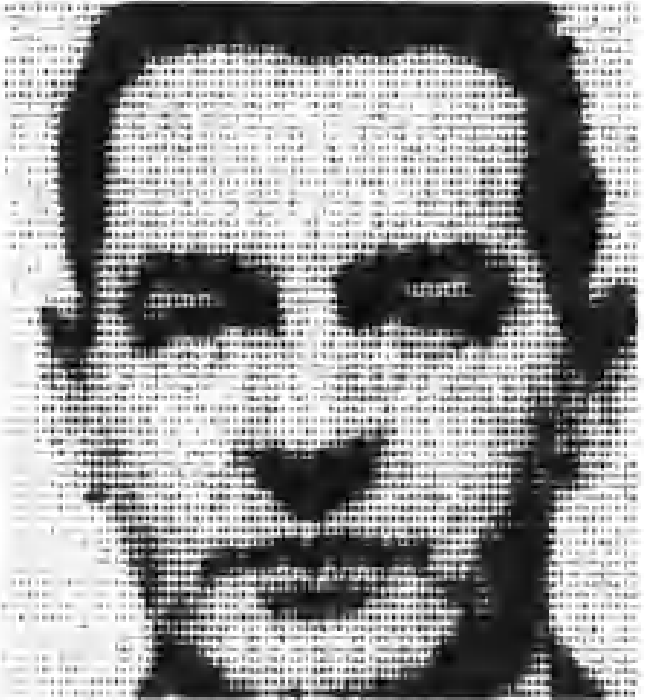
\includegraphics[width=\textwidth]{img/kohonenA.png}
         \caption{Stored vector}
         \label{kohonenA}
     \end{subfigure}
     \hfill
     \begin{subfigure}[b]{0.3\textwidth}
         \centering
         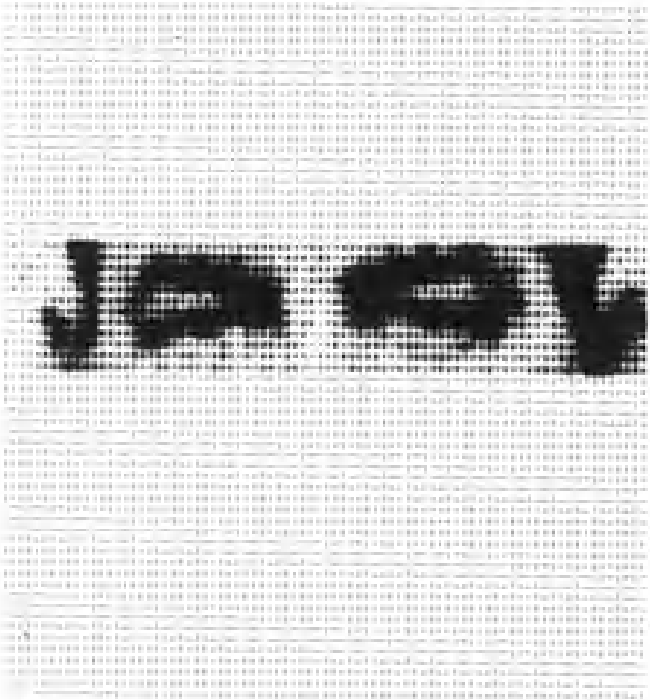
\includegraphics[width=\textwidth]{img/kohonenB.png}
         \caption{Cue vector}
         \label{kohonenB}
     \end{subfigure}
     \hfill
     \begin{subfigure}[b]{0.3\textwidth}
         \centering
         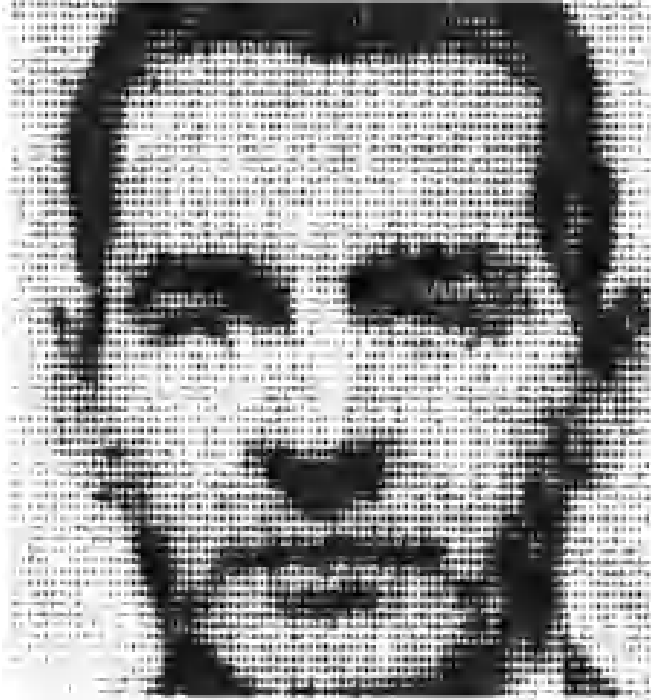
\includegraphics[width=\textwidth]{img/kohonenC.png}
         \caption{Retrieved vector}
         \label{kohonenC}
     \end{subfigure}
        \caption{Example of associative retrieval. A memory that stores 160 different pictures of faces, when given a small snippet containing just the eyes, is able to retrieve the original image. \textbf{(a)} One example out of the 160 images stored in the memory. \textbf{(b)} The cue vector that is used as input to the retrieval process. \textbf{(c)} The retrieved vector that is obtained after the memory computes its final state. Adapted from \cite{kohonen2012self}, original study in \cite{kohonen1977principle}.}
        \label{fig:kohonen}
\end{figure}

When the AM receives as input a \textit{cue vector} $\tilde{\mathbf{x}}$, each neuron of the network will compute its dendritic potential $s_{j}$.
\begin{equation}
    s_{j}=\sum_{i=1}^{m} W_{i j} \tilde{x}_{i}
\end{equation}

Notice that this step can be parallelized since each neuron works independently of the others.

Next, each neuron computes its output $\hat{y}_j$ by applying a \textit{transfer function} $f$, with threshold $\theta_j$, to its previously computed dendritic potential.

\begin{equation}
    \hat{y}_{j}=f\left(s_{j},\theta_j\right)
\end{equation}
The \textit{transfer function} $f$ usually takes the form of a \textit{step function}, like the \textit{Heaviside} function described in equation \ref{eqn:heaviside}. The choice of the \textit{threshold} parameter $\theta$, which controls the sensitivity of activation, is of extreme importance: an appropriate rule can greatly enhance the memory's performance, allowing for the storage of more vectors with no penalty on the retrieval quality. If $\theta$ is set too high, very few neurons will activate, even with strong dendritic potential. On the other hand, if $\theta$ is set too low, many neurons will activate in a "false-positive" manner. A well-suited value for $\theta$ will ensure that the correct amount of correlations between neurons and the \textit{cue vector} are detected, resulting in an error-free \textit{retrieval}.

Some rules define a global \textit{threshold} $\theta_j = \theta_{global} \mid j=1, \ldots, n $ shared by all neurons, others rely on each neuron to store its activation threshold locally.

After all the neurons have computed their state $y_j$, the state of the whole network represents the retrieved vector $y$. When the retrieval process ends here, it is called \textit{one-step retrieval} which occurs on feed-forward AMs. However, certain AMs, like the Hopfield Network \cite{hopfield1982neural}, employ \textit{recurrent} architectures. In such cases, the state $y$ computed in the first step of \textit{retrieval} is fed back into the network as input, and the retrieval process is repeated until convergence. This method is known as \textit{iterative retrieval}.

\subsection{Performance Assessment}
\label{sec:assomem_perf}
The performance metric of associative memories is its \textit{storage capacity}. After all, a memory system is as good as the number of different memories it can hold. Any associative memory can hold a small number of vectors and retrieve them perfectly, but as more vectors are stored, the memory starts to fill up and retrieval becomes imperfect (see figure \ref{fig:kohonen2} for an illustration). If too many vectors are added to the memory it can become saturated and rendered useless, not even able to retrieve the first learned vectors.

\begin{figure}[htbp]
     \centering
     \begin{subfigure}[t]{0.3\textwidth}
         \centering
         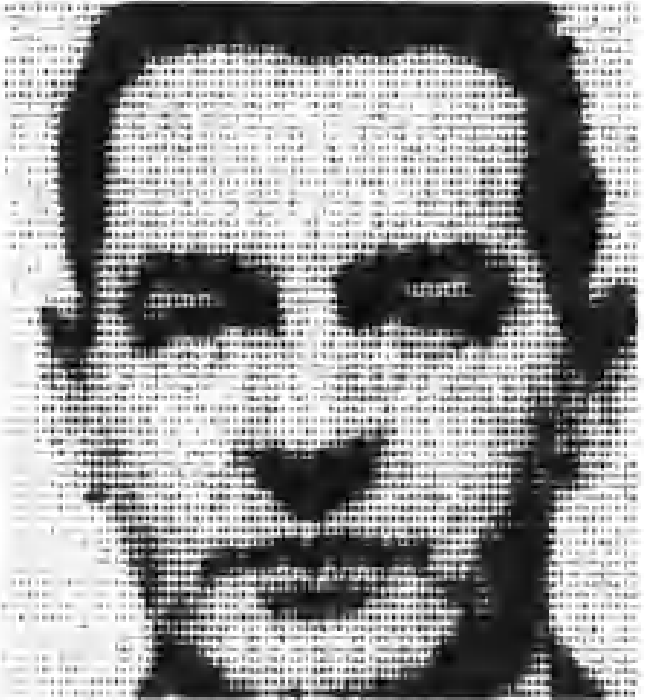
\includegraphics[width=\textwidth]{img/kohonenA.png}
         \caption{Stored vector}
         \label{kohonen2A}
     \end{subfigure}
     \hfill
     \begin{subfigure}[t]{0.3\textwidth}
         \centering
         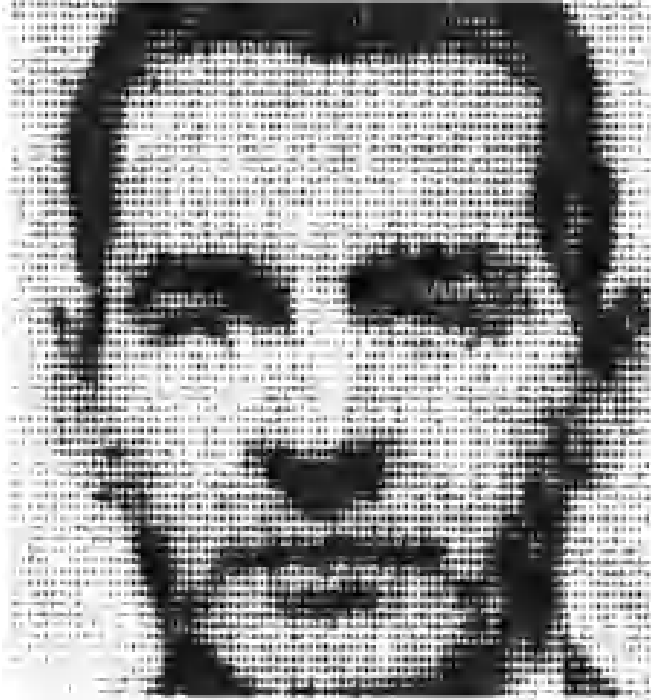
\includegraphics[width=\textwidth]{img/kohonenC.png}
         \caption{Retrieved: memory with 160 vectors}
         \label{kohonen2B}
     \end{subfigure}
     \hfill
     \begin{subfigure}[t]{0.3\textwidth}
         \centering
         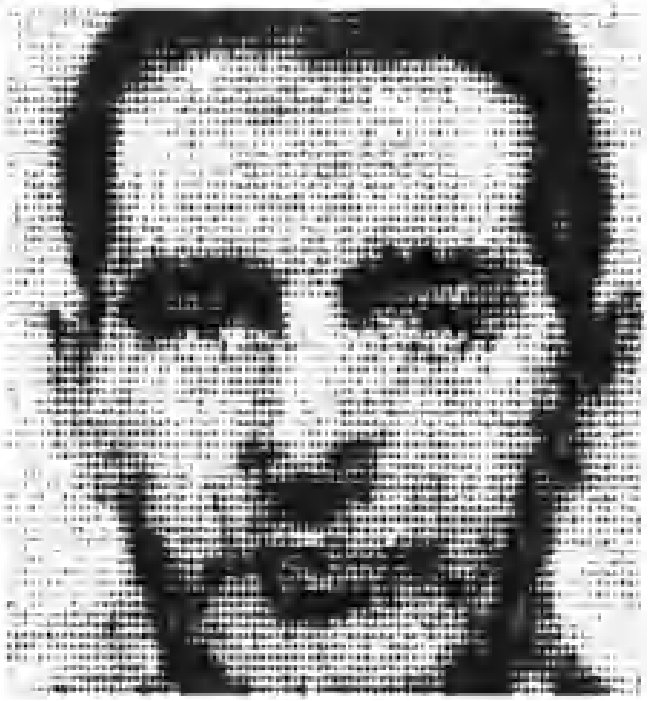
\includegraphics[width=\textwidth]{img/kohonenD.png}
         \caption{Retrieved: memory with 500 vectors}
         \label{kohonen2C}
     \end{subfigure}
        \caption{Effect of the number of stored vectors on retrieval quality. In this experiment, similarly to figure \ref{fig:kohonen}, a small part of the image is used as the cue vector for retrieval. \textbf{(a)} The original vector that is stored in memory. \textbf{(b)} The retrieved vector obtained when the memory is filled with 160 vectors. We can notice some small imperfections in the retrieved image. \textbf{(c)} The retrieved vector obtained when the memory is filled with 500 vectors. The high number of stored vectors is causing a large retrieval error, the retrieved image has noticeable artifacts. Adapted from \cite{kohonen2012self}, original study in \cite{kohonen1977principle}.}
        \label{fig:kohonen2}
\end{figure}
    
Formally, the storage capacity $L$, admitting an \textit{error factor} $\epsilon$ of an AM with $n$ neurons, is the total number of pairs $(x,y)$ that can be stored in memory without experiencing a retrieval error greater than $\epsilon$. Typically described as a function of the size $n$ (number of neurons) of the network.

For example, the Linear Associator (studied independently by \cite{anderson1968memory}, \cite{kohonen1972correlation}, \cite{anderson1972simple}, or \cite{nakano1972associatron}), a very simple AM, had a storage capacity of $L=n$ when storing orthogonal vectors. Another example is the original version of the Hopfield Network, which had a capacity of $L = 0.14n$ for uncorrelated vectors. 
%TODO: rewrite this phrase and mention how AMs are always studied with random noise.
Notice that these theoretical values for the storage capacities of AMs are often studied under ideal scenarios, such as storing uncorrelated or orthogonal vectors. As it turns out, vectors with certain properties are very well suited for storage in AMs, resulting in great storage capacities. However, real-world data typically lacks those properties, which is the main cause for the shortcomings of AMs in practical applications. Finding mechanisms to transform real-world data into "AM-suitable" vectors is the key to unlocking the full potential of AMs. We will discuss the desired properties of vectors in subsection \ref{sec:inputoutput}, and the existing mechanisms to generate them in section \ref{SDRgen}.
%TODO: maybe talk about how the storage capacity improves for very large matrices. Compare storage capacity of large AMs to listing memories.


\section{Willshaw network}
\label{sec:wn}
The Willshaw Network (WN) \cite{willshaw1969non} is a one-layer, feed-forward ANN that performs \textit{auto} and \textit{hetero-association} of binary vectors.

Originally named \textit{Lernmatrix} by its creator Karl Steinbuch in the 1950s \cite{steinbuch1961lernmatrix}, the biologically-inspired model was one of the pioneer implementations of ANNs.
The Lernmatrix became more popular in the following decade when it was studied through a mathematical/biological lens by D. Willshaw \cite{willshaw1969non}. Thus becoming known as the \textit{Willshaw Network}. Despite its simplicity, both in its binary nature and in its learning/retrieval rules, the WN is great artificial memory, capable of storing great amounts of vectors.

\subsection{Architecture}
\label{sec:wn_arch}
The WN is composed by one layer of $n$  \textit{units}, also referred to as \textit{neurons}. Each neuron has $m$ binary connections to the other neurons.
The network is represented as a binary matrix $W$:
\begin{equation}
W_{ij} \in \{0,1\} : i=1, \ldots, m ;  j=1, \ldots, n
\end{equation}
The dimensions $m$ and $n$ are given by the fixed sizes of the \textit{question} and \textit{answer} vectors, respectively. Notice that, in an auto-association task, $W$ will be a square matrix of size $(n \times n)$. 
This matrix defines the absence/presence of connections between neurons. A connection between two neurons $i$ and $j$ is formed during training when a local Hebbian rule detects a correlation between the positions $i$ of a \textit{question} vector, and the position $j$ of an \textit{answer} vector.

Additionally, each neuron has a local threshold $T_n$, used in the last step of retrieval as the parameter of the \textit{transfer function}. A schematic view of the network can be seen in figure \ref{WN1}.

\begin{figure}[htbp]
     \centering
     \begin{subfigure}[t]{0.49\textwidth}
         \centering
         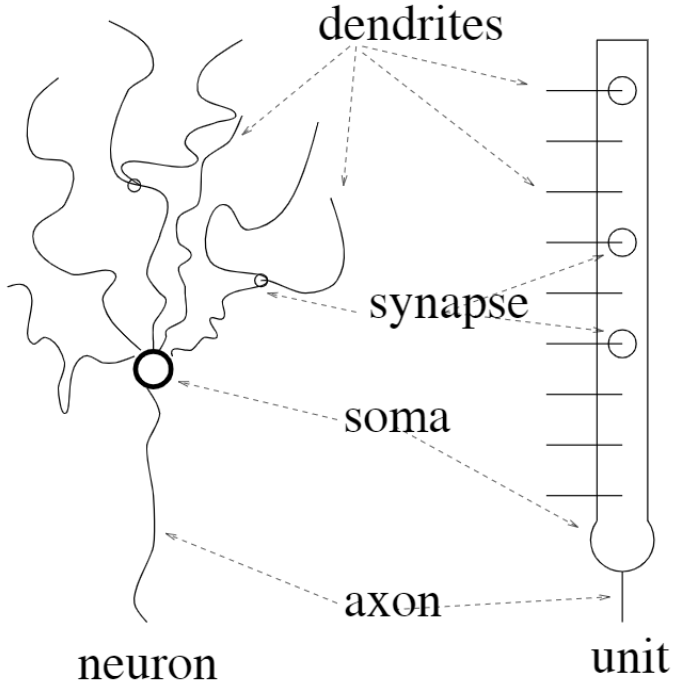
\includegraphics[height=4cm]{img/wichert2.png}
         \caption{Biological vs Artificial neuron.}
         \label{WN2}
     \end{subfigure}
     \hfill
     \begin{subfigure}[t]{0.4\textwidth}
         \centering
         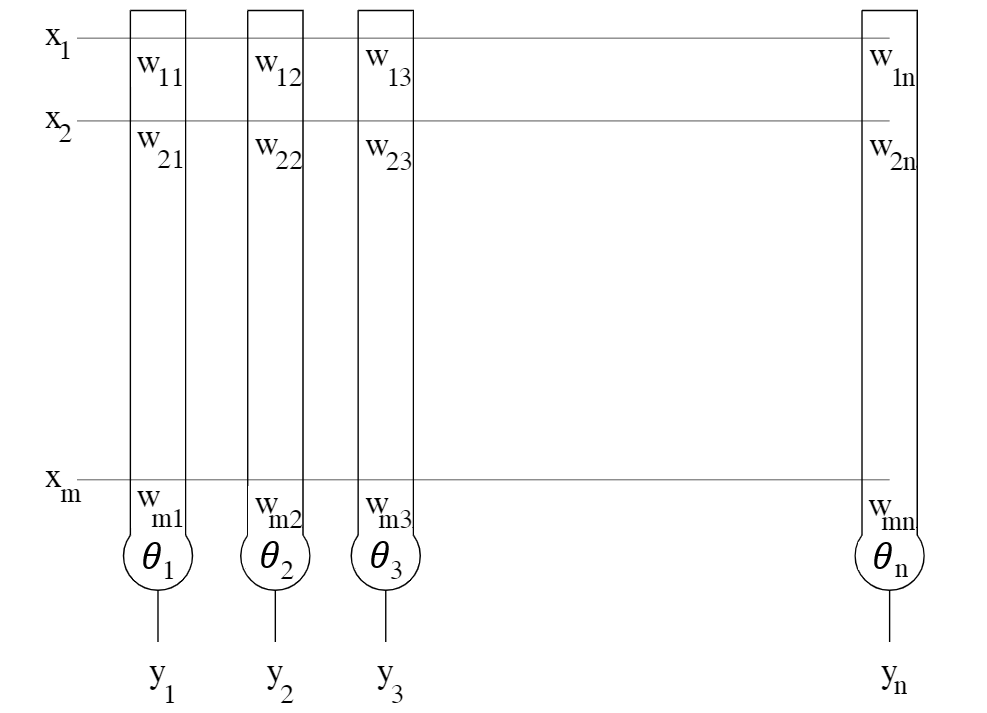
\includegraphics[height=4cm]{img/wichert1.png}
         \caption{Willshaw Network schematic.}
         \label{WN1}
     \end{subfigure}
     \hfill
        \caption{Neurons of the Willshaw Network. \textbf{(a)} A side-by-side comparison of a biological neuron (left) and a Willshaw Netork's unit (right). \textbf{(b)} A schematic representation of a \textit{Willshaw Nework}. Composed of a set of  $n$ vertical units which represent a simple model of a real biological neuron. Each neuron has $m$ weights, which correspond to the synapses and dendrites in the real neuron. In this Figure they are described by $w_{ij} \in  \{0,1\}$ where $1\leq i \leq m$ and $1 \leq j \leq n$. $\theta_j$ is the threshold of each neuron $j$. Adapted from \cite{wichert2020principles}.}
        \label{fig:WN}
\end{figure}


\subsection{Biological plausibility}
\label{sec:wn_bio}
The human brain is the most intelligent system that we know of. Understanding the brain and implementing its mechanisms is the ultimate goal of Biologically inspired models. AMs are examples of such models as they try to imitate the associative capabilities of the brain.

The \textit{Lernmatrix/Willshaw Network}'s development has always been guided by biology and neuroscience. The original purpose of the model was to study psychological conditioning \cite{steinbuch1961lernmatrix,steinbuch1965automat}.
The model was later analyzed by Palm \cite{palm1982neural} on its ability to implement assemblies of cells under the Hebbian framework \cite{hebb2005organization}.
Furthermore, the network's units are artificial neurons \cite{mcculloch1943logical} modeled after their biological counterparts (see figure \ref{WN2}). Finally, the neural energy efficiency of the model has been analyzed \cite{laughlin2003communication,lennie2003cost}.

All in all, the WN, while far from a replica of the brain, is heavily biologically inspired. Consequently, its application in practical scenarios is significant, since it might give us interesting insights into our still limited understanding of the brain. 

\newpage
\subsection{Learning and Retrieval rules}
\label{sec:wn_rules}
The WN is completely binary: its inputs $x$, outputs $y$, and weight matrix $W$ are binary. Consequently, its learning and retrieval rules are simple.
\newline

For the next equations, let us use the following convention:
\begin{itemize}
    \item The $n$ neurons of the network are referenced with the index $j$.
    \item The $m$ connections of each neuron are referenced with the index $i$.
    \item The weight matrix $W$ has $m$ rows and $n$ columns (see figure \ref{WN1}), and it is indexed as $W_{ij}$.
\end{itemize}

For the learning rule, given a set of $M$ pairs $(x,y)$, the weight matrix $W$ is computed with the following binary learning rule: 
\begin{equation}
W_{i j}=\min \left(1, \sum_{\mu=1}^{M} x_{i}^{\mu} y_{j}^{\mu}\right)
\label{eqn:wn_lrn}
\end{equation}
\newline

The retrieval of a cue vector $\tilde{x}$ is performed in two steps. First the dendritic potential $s$ is computed in each neuron:
\begin{equation}
\label{eqn:dendritic}
    s_{j}=\sum_{i=1}^{m} W_{i j} \tilde{x}_{i}
\end{equation}
Secondly, the retrieved vector $\hat{y}$ is computed for all neurons:
\begin{subequations}
\label{eqn:wn_ret}
\begin{equation}
    \theta_{j}=\max _{1 \leq i \leq n} s_j
\label{eqn:wn_ret_theta}
\end{equation}
\begin{equation}
\label{eqn:wn_ret_y}
    \hat{y}_{j}=H\left(s_{j}-\theta_{j}\right)
\end{equation}
\end{subequations}
Equation \ref{eqn:wn_ret_theta} is known as\textit{ soft thresholding}. It defines a neuron-local strategy for the transfer function's activation threshold $\theta$. This strategy was used by Palm, Schwenker, Sommer, and Strey in \cite{palm1992information,gunther1997neural}. Soft thresholding is the best performing strategy for the WN. Alternatively, one could use a simpler strategy, such as \textit{hard thresholding}, where $\theta$ is set globally to the number of ones in the cue vector: ($\theta_j=\sum_{i=1}^{m} \tilde{x}_i \mid j=1, \dots , n)$.
In equation \ref{eqn:wn_ret_y}, $H$ refers to the \textit{Heaviside} step function described in equation \ref{eqn:heaviside}.

Equations \ref{eqn:wn_lrn} to \ref{eqn:wn_ret} fully specify the computations required to operate a WN. Next, we provide a simple example to better illustrate the learning and retrieval process.
\newpage
\subsubsection{Example of Willshaw Learning and Retrieval}
\label{sec:wn_example}

Consider that we want to store two patterns in \textit{auto-association} in a WN:

$x^{1} = (0,0,1,1)$

$x^{2} = (1,1,0,0)$
\newline
Since this is an \textit{auto-association} task, we have $y=x$:

$y^{1} = (0,0,1,1)$

$y^{2} = (1,1,0,0)$
\newline
\newline
The \textbf{learning step} is done by applying the rule defined in equation \ref{eqn:wn_lrn}:
\newline

$W_{i j}=\min \left(1, \sum_{\mu=1}^{M} x_{i}^{\mu} y_{j}^{\mu}\right)$
$=\left[\begin{array}{llll}
1 & 1 & 0 & 0 \\
1 & 1 & 0 & 0 \\
0 & 0 & 1 & 1 \\
0 & 0 & 1 & 1 
\end{array}\right]$
\newline

Notice how $W$ is a square and symmetrical matrix, which is always the case in \textit{auto-association} tasks.
\newline
\newline
Now, consider that we query the network with the following \textit{cue} vectors:

$\tilde{x}^{1} = (1,0,1,1)$ - a noisy version of the patter $x^{1}$. 

$\tilde{x}^{2} = (1,0,0,0)$ - an incomplete version of  the patter $x^{2}$.
\newline
\newline
The \textbf{retrieval step} begins by applying equation \ref{eqn:dendritic} to each \textit{cue}, resulting in the following dendritic potentials:

$s^1=(1,1,2,2)$

$s^2=(1,1,0,0)$
\newline
Next, we can determine the local activation thresholds $\theta$ using equation \ref{eqn:wn_ret_theta}:

$\theta^1=2$

$\theta^2=1$
\newline
Finally, we use equation \ref{eqn:wn_ret_y} to obtain the \textit{retrieved vectors}:

$\hat{y}^1 = H((1,1,2,2) - 2) = H(-1,-1,0,0) = (0,0,1,1) = x^1$

$\hat{y}^2 = H((1,1,0,0) - 1) = H(0,0,-1,-1) = (1,1,0,0) = x^2$
\newline

Notice how the memory was able to perfectly reconstruct the original vectors $x^1$ and $x^2$ when corrupted versions of them were used as \textit{cues}. 

The process that is illustrated by this simple example with 4-dimension vectors is the same process that is depicted in figure \ref{fig:kohonen}, where the vectors are now large binary arrays of pixels that represent black and white images.
\newpage

\section{Vectors}
\label{sec:inputoutput}
The inputs and outputs of an AM are vectors (also commonly referred to as patterns). Here, we formally describe what vectors are, and what are their interesting properties in the context of AMs.
\subsection{Definition}
\label{sec:inputoutput_def}
An $n$-dimensional vector $x$ is a collection of  $n$ components $x_i$. The type of components that constitute the vector will determine the AM's function:
\begin{enumerate}
    \item Continuous vectors: function approximation or interpolation
    \item Continuous and finite vectors: classification and recognition
    \item Discrete vectors: classification and memory
\end{enumerate}
In the cases of \textit{hetero} and \textit{auto-association} tasks, AMs typically use the third category:\textit{ discrete vectors}. More specifically, the AMs that are purely intended for association tasks deal with discrete \textit{binary} vectors.

An $n$-dimensional \textit{binary} vector $x$ is a collection of size $n$ where each component $x_i$ can only take one of two values: $x_i \in \{ a,b \} \mid i=1, \dots,n$.
Any two literals or numbers can be used, for instance $a=W$ for white pixels, and $b=B$ for black pixels. More commonly, discrete values are used such as $(a,b)=(-1,+1)$ in the original Hopfield Network, or $(a,b)=(0,1 )$ in the Willshaw Network.
\newline

From this point on, we will focus solely on binary vectors, and the convention $(a,b)=(0,1)$ is adopted.

\subsection{Properties of binary vectors}
\label{sec:inputoutput_propbin}
When using \textit{binary} vectors, the amount of 0s (inactive bits) and 1s (active bits) in the vector is a key property.
Given a vector $x$ of size $n$, let the ratio $p$ denote the relative proportion of 1s in the vector:
\begin{equation}
    p = \frac{\text{number of 1s}}{\text{size of x}} =  \frac{\sum\limits_{i=1}^k{x_i}}{n}
\end{equation}
Another useful way to interpret $p$ is the probability that a given position of the vector, chosen at random, is active.

Concerning the amount of 1s in a binary vector, it can be classified as \cite{palm1996associative}:
\begin{itemize}
    \item \textit{Singular} if, out of the $n$ bits, there is a single 1 and the remaining $n-1$ bits are 0s. This type of representations is also referred to as \textit{one-hot encoding}.
    \item \textit{Sparse} if the relative amount of 1s is very small ($p\ll0.5$). In mathematical terms, a\textit{ sparse }vector obeys: $\lim _{n \rightarrow \infty} p=0$. For example, a \textit{singular} vector has: $\lim _{n \rightarrow \infty} p = $ $ \lim _{n \rightarrow \infty} \frac{1}{n} = 0$ which is \textit{sparse}.
    \item \textit{Non-sparse} if the relative amount of 1s is away from zero. In other words, a \textit{non-sparse} vector has: $\lim _{n \rightarrow \infty} p=K$, with $K \neq 0$. For instance, \textit{random} binary vectors have approximately as many 0s as 1s, consequently we have: $\lim _{n \rightarrow \infty} p = $ $ \lim _{n \rightarrow \infty} 0.5 = 0.5 \neq 0$ which is \textit{non-sparse}.
\end{itemize}
Associative memories perform better when storing sparse vectors. For instance, a Hopfield Network can store L = 0.72n sparse vectors \cite{gardner1988space}. But in the case of non-sparse vectors, the capacity drops to L = 0.14n \cite{hopfield1982neural}. This trend is common amongst other AMs such as the Wilshaw Network.
\newline

Additionally, in the context of the entire set S (equation \ref{eqn:S}) of vectors to be stored in memory, the desired properties of S are the following:
\begin{itemize}
    \item $S$ should be \textit{uniformly sparse}, meaning that all vectors in $S$ should have similar sparsity (besides also being individually sparse).
    \item $S$ should be \textit{distributed}, meaning that all the $n$ positions of the vectors are uniformly active across all the vectors in $S$.
\end{itemize}

The property of \textit{distribution} is better understood visually. Let us introduce a new definition to better illustrate this property:
\newline
For the set of vectors $S$, and a given position of the vectors $i$, let $P$ be the ratio of vectors $x$, in $S$, that have a 1 in the $i$th position.
\begin{equation}
\label{eqn:P}
    P = \frac{1}{M}\sum_{\mu=1}^{M}x^{\mu}_i
\end{equation}
A \textit{distributed} set of vectors is one that has a similar $P$ value for all the $n$ positions of the vectors in it. Figure \ref{fig:sparse} illustrates the \textit{distribution} and \textit{sparsity} properties of binary vectors.

When the training vectors meet the criteria of \textit{sparsity}, \textit{uniform sparsity}, and \textit{distribution}, we can refer to them as \textit{Sparse Distributed Representations}. This kind of vector can very efficiently be stored in AMs, allowing for great storage capacities.

\begin{figure}[h]
    \centering
    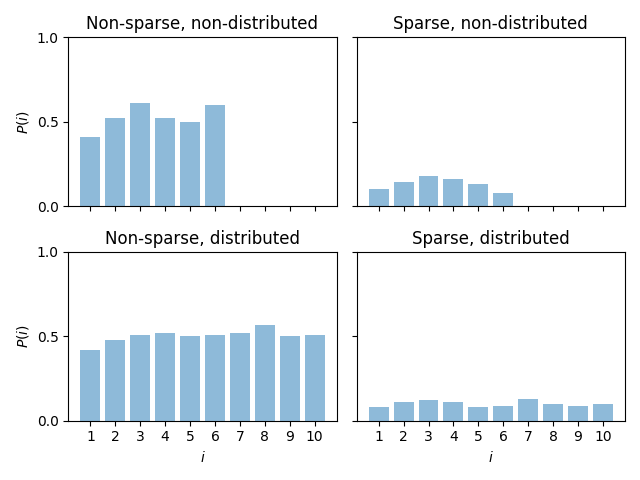
\includegraphics[width=0.8\textwidth]{img/sparse.png}
    \caption{The properties of a binary vector training set $S$ (equation \ref{eqn:S}) described with $P$ (equation \ref{eqn:P}). In this example we are storing 10-dimension vectors in the AM. The x-axis represents the 10 positions $i$ of the vectors. The y-axis represents $P(i)$, which is the probability that we find a 1 in the $i$th position of a vector of $S$, picked at random. Two properties of $S$ (sparsity and distribution) are shown in all 4 possible combinations. \textbf{(top row)} Non-distributed: the 1s in $S$ are not equally distributed in the 10 dimensions. \textbf{(bottom row)} Distributed: the 1s in $S$ are equally distributed in the 10 dimensions. \textbf{(Left column)} Non-sparse: There is a high amount of 1s in $S$ \textbf{(Right-Row)} Sparse: The amount of 1s in S is limited.}
    \label{fig:mesh1}
\label{fig:sparse}
\end{figure}
\subsection{Sparse Distributed Representations}
\label{sec:inputoutput_sdr}
% What are SDRs, biological plausibility
Our brains "(...) represent information using a method called \textit{Sparse Distributed Representations}, or SDRs." \cite{Hawkins-et-al-2016-Book}. Neuroscience has shown that information in the brain is represented by the sparse activation of groups of neurons in the cortex \cite{olshausen1996emergence}. In this way, SDRs are biologically plausible informative representations.

% They sacrifice compactness for information
This kind of representation is restricted by the \textit{sparsity} and \textit{distribution} properties. On one hand, these restrictions make SDRs less compact representations (more bits are required), but on the other hand, these same restrictions give rise to vectors where each bit captures a relevant detail/feature of the training set $S$.
% compression property
Since the vectors are sparse, only the prime features of each training example will be selected to be active in the vector. In such a way, SDRs also act as compressions.

%Explain why they are informative
The most important property of SDRs is that each of its bits has meaning \cite{Hawkins-et-al-2016-Book}. If two representations of different items share an active bit in the same position, it means that the items themselves share some semantic similarity. The information is carried in the representation itself, not stored externally. This property is what makes SDRs informative representations.
% why this is good for AMs
Since AMs are \textit{content addressable} memories, i.e. they handle inputs as content/information, they benefit immensely from this SDR property.

% contrast between SDRs and dense representations
The informative nature of SDRs becomes evident when we compare SDRs with the dense representations commonly found in computers. A dense representation is a non-informative compact way to encode information. It uses the least possible amount of bits to assign a unique code to each item. A table containing the mapping between the codes and the items is established and this table must be looked up to make sense out of the representations. The information resides in the table, not the codes.

\subsubsection{Example: Encoding numbers}
\label{sec:inputoutput_example}
Let us compare two different approaches for encoding numbers: a dense representation and an SDR.

The ASCII representation for character encoding is dense. It uses all the $2^7$ possible combinations of 7 bits to code 128 different characters. The mapping between codes and characters is stored in the ASCII table (see table \ref{tab:ascci}). Every character is assigned a unique 7-bit code. The individual bits of the code carry no meaning. Only the complete combination of the 7 bits allows us to determine which character is being encoded. All the information is stored in the table, not the codes.

\begin{center}
\captionof{table}{Example of entries in the ASCII table.}
 \label{tab:ascci}
 \begin{tabular}{||c c c ||} 
 \hline
 character & code(dec) & ASCII code \\ [0.5ex] 
 \hline\hline
 1 & 49 & 0110001 \\
 \hline
 2 & 50 & 0110010 \\
 \hline
 3 & 51 & 0110011 \\
 \hline
 $\dots$ &  $\dots$ &  $\dots$\\ 
 \hline
 6 & 54 & 0110110 \\ [1ex]
 \hline
\end{tabular}
\end{center}

Now, let us consider an SDR for number encoding. Figure \ref{fig:SDR_number_encoder} depicts a simple encoder that mimics how the human cochlea encodes frequency in the inner ear. The representations produced by this encoder are known as the \textit{thermometer encoding},  which are sparse and distributed (see table \ref{tab:sdr} for examples). The main idea is that the several bits in the representation correspond to sensors that activate for specific values. A value will activate both the corresponding sensor and its neighbors, thus producing informative representations. 

\begin{figure}[h]
    \centering
    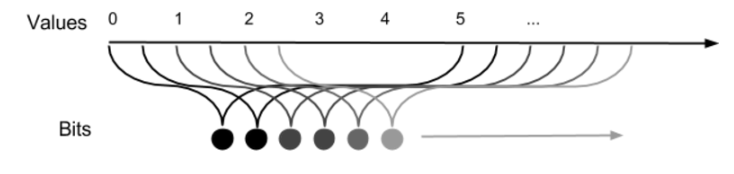
\includegraphics[width=0.9\textwidth]{img/SDR_number_encoder.PNG}
    \caption{An SDR encoder. Each bit in the representation responds to a range of values that overlaps with its neighbors. Here, the representations have 105 bits, and only 6 are active at a time, guaranteeing a sparsity of approximately 5\%. This encoder can code numbers from $0$ to $100$. Notice how the encoder will produce distributed codes, i.e. the entire 105 bits will be used uniformly (see figure \ref{fig:sparse})). Adapted from \cite{Hawkins-et-al-2016-Book}.}
\label{fig:SDR_number_encoder}
\end{figure}

\begin{center}
\captionof{table}{Example of entries in an SDR encoding strategy. See figure \ref{fig:SDR_number_encoder} for the encoding strategy.}
\label{tab:sdr}
 \begin{tabular}{||c c||} 
 \hline
 character & 105-bit code \\ [0.5ex] 
 \hline\hline
 6 & 1111110000000...000 \\
 \hline
 7 & 0111111000000...000 \\
 \hline
 8 & 0011111100000...000 \\
 \hline
 $\dots$ & $\dots$\\
 \hline
 13 & 0000000111111...000 \\
 \hline
\end{tabular}
\end{center}

Notice how the thermometer encoding carries information in its bits. Small numbers will use the left side of the vector while large numbers will use the right side. Two numbers that are close in value will share bits in their representation (for example "6" and "7" have 5 overlapping 1s), while numbers that are far apart will not share any bits (for example "7" and "13" share no active bits).
In the ASCII representation, overlaps between different representations have no meaning. The representation of a "2" differs in a single bit to both the representation of a "3", and a "6". Overlapping bits are just coincidences. 

The thermometer encoding is also resistant to noise: If a few 1s are removed or added to an existing representation, we can still know if the number is large or small by looking at the overall position of the active bits. In the ASCII representation, switching a single bit completely alters the information.

The informative nature of SDRs also means that we can compare two representations and assess their similarity with no knowledge of the domain or the task.

From this example, we can observe how bits carry information in SDRs, and how they don't in dense representations.
% mention how we can still compare SDRs without knowing what the domain is, and how they are naturally regularizers
This great property comes at the cost of size. While the ASCII representation uses 7 bits, this SDR used 105. In practice, SDRs are implemented with pointer structures that only stores the active bits.

% real word data is dense; we need to find mechanisms that perform feature extraction to produce SDRs
\subsection{The sparse coding problem}
\label{sec:inputoutput_problem}
Associative memories can greatly increase their capacity if they store SDRs. However, it turns out that most real-world data is not naturally sparse (see figure \ref{fig:mnist}). To successfully apply AMs to real-world problems, we must find prescriptions that transform dense representations into SDRs. This problem is known in the literature as \textit{the sparse coding problem}, and it has been studied in many different domains by different researchers. In the end, it boils down to the idea of extracting relevant features from the available data to compress it into a sparse representation. In the upcoming section, we will go over some of the existing solutions for the \textit{sparse coding problem}.

\begin{figure}[h]
    \centering
    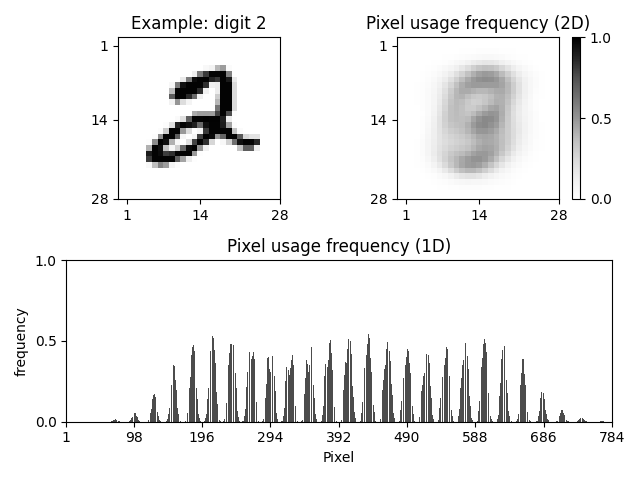
\includegraphics[width=0.9\textwidth]{img/MNIST.png}
    \caption{ Example of the lack of sparsity and distribution on real-world data. Here, the MNIST dataset \cite{lecun1998mnist} is used. The dataset contains 70,000 images of hand-written numbers, drawn by 250 different writers. Each image is 28 pixels wide and 28 pixels high, totaling 784 pixels per image.
    \textbf{(top-left)} One single example out of the 70,000 images in the dataset. 
    \textbf{(top-right)} The relative frequency (encoded with colour) at which each pixel is used. 
    \textbf{(bottom)} The same pixel frequency depicted in the top-right picture, visualized in a single horizontal axis. Notice how the data is neither sparse nor distributed (compare with figure \ref{fig:sparse}).}
\label{fig:mnist}
\end{figure}

\section{Sparse Encoding Prescriptions}
\label{sec:prescriptions}

Strategies that transform natural data into SDRs are required to solve the sparse
coding problem. Here, we refer to such strategies as \textit{encoding functions}.
The desired properties of an \textit{encoding function} are \cite{Hawkins-et-al-2016-Book}:
\begin{itemize}
    \item Semantically similar data should result in SDRs with overlapping active bits.
    \item The same input should always produce the same SDR as output.
    \item The output should have the same dimensionality (total number of bits) for all inputs.
    \item The output should have similar sparsity for all inputs and have enough one-bits to handle noise and subsampling.
\end{itemize}

An important aspect of Artificial Intelligence (AI) models is their amount of predefined \textit{structure}. AI models can be broadly divided into two categories: those that use "a priori" knowledge in their structure (\textit{Nativism}), and those that don't (\textit{Connectionism}).
The first is a traditional approach \cite{newell2007computer}, where the knowledge about the domain of the problem is used to design comprehensible solutions.
The second is a more recent approach, focused on building general algorithms (usually Neural Networks) that can learn with minimal assumptions/biases about the problem.
Due to the huge diversity of available AI techniques, there isn't a binary way to classify models in terms of their structure, instead, there is a wide spectrum.
In the \textit{Nativism} end of the spectrum, we have techniques such as first-order logic models \cite{mitchell1997machine} where the model's structure is strictly predefined.
On the other end, we have \textit{Connectionism} techniques, such as the multi-layered perceptron (MLP) \cite{hornik1989multilayer}, where the structure is not imposed beforehand, but learned through the weights of the model.
In between these two extremes, there is a large diversity of models that have both Nativism and Connectionism aspects. From Deep Blue \cite{campbell2002deep}, the chess machine that beat the world champion with an efficient tree search, to a deep reinforcement learning model that learns to play different video games using only the raw pixels as input  \cite{mnih2015human}.

In the following section, we will present two examples of encoding functions, a \textit{Nativism} approach, and a \textit{Connectionism} approach.

\subsection{What-Where Encoding (Nativism Approach)}
\label{sec:prescriptions_WW}
``Vision allows humans to perceive and understand the world surrounding them, while computer vision aims to duplicate the effect of human vision by electronically perceiving and understanding an image." \cite{sonka2014image}
The field of Computer Vision has been highly connected to biology \cite{marr1982vision} since the 1980s. The field's Holy Grail is to build a model that performs as well as the human brain. For this reason, many \textit{Nativism} models, that implement our biological knowledge of vision, arise in image processing tasks.

In \cite{sa2020storing}, Sa-Couto \& Witchert propose an \textit{encoding function} that maps visual patterns into informative binary vectors. The \textit{Nativist} model is biologically inspired, using similar ideas to those of the \textit{Neocognitron} \cite{fukushima1988neocognitron}. The \textit{Neocognitron} is a direct implementation of Hubel \& Weisel's Nobel-Prize-winning theory of the mammalian visual cortex \cite{hubel1962receptive}, and it is the precursor of the widely popular Convolutional Neural Networks (CNNs) \cite{lecun1989backpropagation}.

The goal of the authors was to implement a one-way, sparse encoding function for visual patterns that could be used to preprocess data in classification tasks. The resulting representation were SDRs, so the authors experimented on the Willshaw Network: This Associative memory will have a better storage capacity if the representations it receives are informative. Knowing this, we can evaluate the quaility of the encoding prescription as a whole by monitoring the retrieval score of a WN that stores the representations.

Experiments on noisy and noiseless versions of visual patterns (MNIST dataset \cite{lecun1998mnist}) were performed. Using an AM to store such a large collection of natural data is traditionally a very hard task for these models, and as expected, retrieval was imperfect. For this reason, the authors proposed a novel error measure that utilized the labels of the patterns. The results show that the codes produced by this strategy are effectively compressing the information in the patterns, so much so that a very simple 1 nearest-neighbor classifier can perform classification when trained on the outputs of a WN that stores the compressions in auto-association.
\newline

\begin{figure}[h]
    \centering
    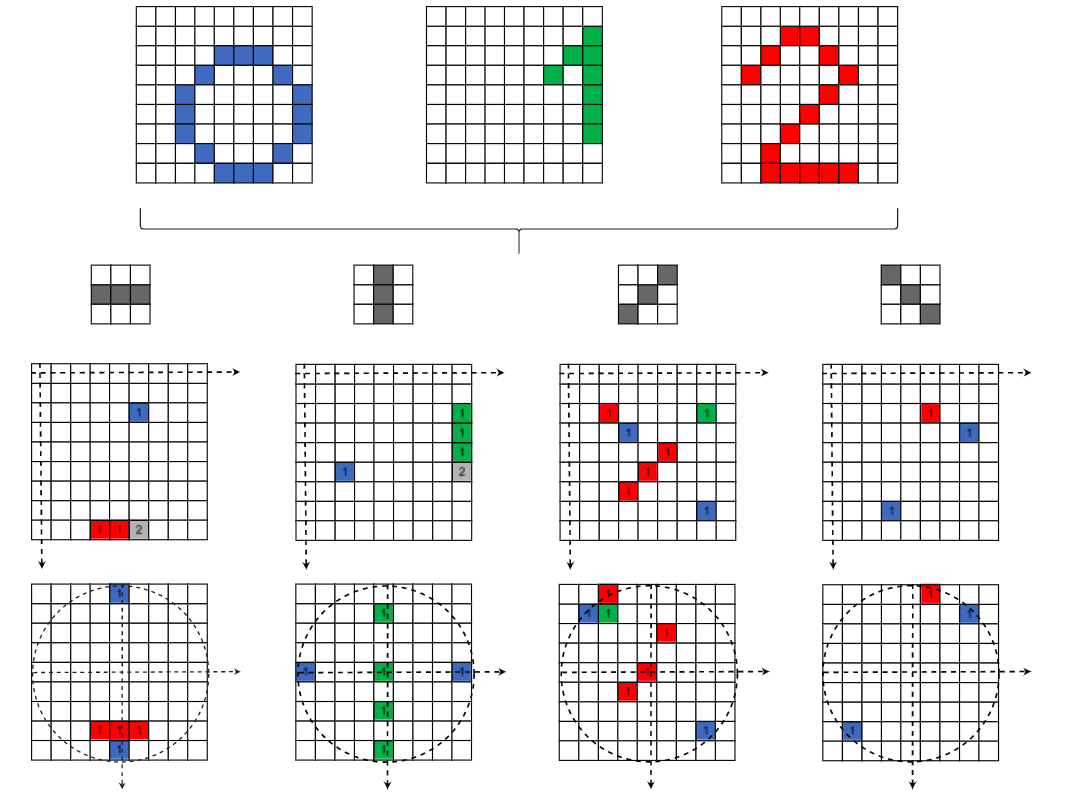
\includegraphics[width=0.9\textwidth]{img/sacouto1.png}
    \caption{Overview of the strategy that transforms visual patterns of digits
    into sparse and distributed codes. The first step is local feature
    extraction. Each feature is depicted as a 3×3 window with an oriented line.
    Each image is parsed with a sliding window, and each occurrence of each
    feature is signaled at the middle layer. The positions where these signalings
    occur refer to a fixed coordinate system. The second step maps these
    positions to an object-dependent, radius one polar coordinate system. Note
    that the final representation (bottom row) corresponds to three distinct
    representations (one for each of the digits). Adapted from \cite{sa2020storing}.}
\label{fig:sacouto1}
\end{figure}

An overview of the encoding function can be seen in figure \ref{fig:sacouto1}. The strategy has two main steps:

\textbf{The retinotopic Step}: A convolution-like layer \cite{lecun1995convolutional} of units that act as receptive fields are locally connected to the input layer. These receptive fields detect and extract the most relevant visual features of the patterns. These features are determined beforehand with the unsupervised K-means algorithm \cite{lloyd1982least,wu2008top}. This layer performs information compression by establishing a many-to-one relationship between groups of pixels and receptive units. In this way, it transforms the dense representation presented in the input layer into a sparse representation.

\textbf{The Object-Dependent Step}: The fixed coordinate system of the representations is turned into a one-radius, polar, object-centered one. This object-oriented transformation is known to occur on mammalian brains \cite{chafee2007representing}. For this step, only the radius and center of each object need to be measured, no learning is required. This operation provides invariance to size and position, and in turn, also makes the resulting representations well-distributed since the features detected in the previous step will be mapped uniformly into all the dimensions of the object space. 

\subsection{Autoencoders (Connectivism approach)}
\label{sec:prescriptions_AEs}

%The structure of an ecoder is made up of two modules:The \textbf{encoder} $f$ transform patterns $x$ of a dataset into new representations $h$; and the \textbf{decoder} $g$ transform the representations $h$ back into the original patterns $x$ with minimal loss (see figure \ref{fig:autoencoder} for an illustration).

An \textit{autoencoder} (AE) is a lossy data compression algorithm that can be used to generate SDRs. It is implemented as a feed-forward ANN with two modules: The \textbf{encoder} which transforms the original inputs $x$ into compressed representations $h$; and the \textbf{decoder} which takes the compressed representations $h$, and creates reconstructions $r$ (see figure \ref{fig:autoencoder} for an illustration). The compression and decompression functions are learned automatically from unlabeled data rather than hand-engineered by a human. Additionally, the AE also has a loss function $L(x,r)$ that measures the reconstruction error.

\begin{figure}[h]
    \centering
    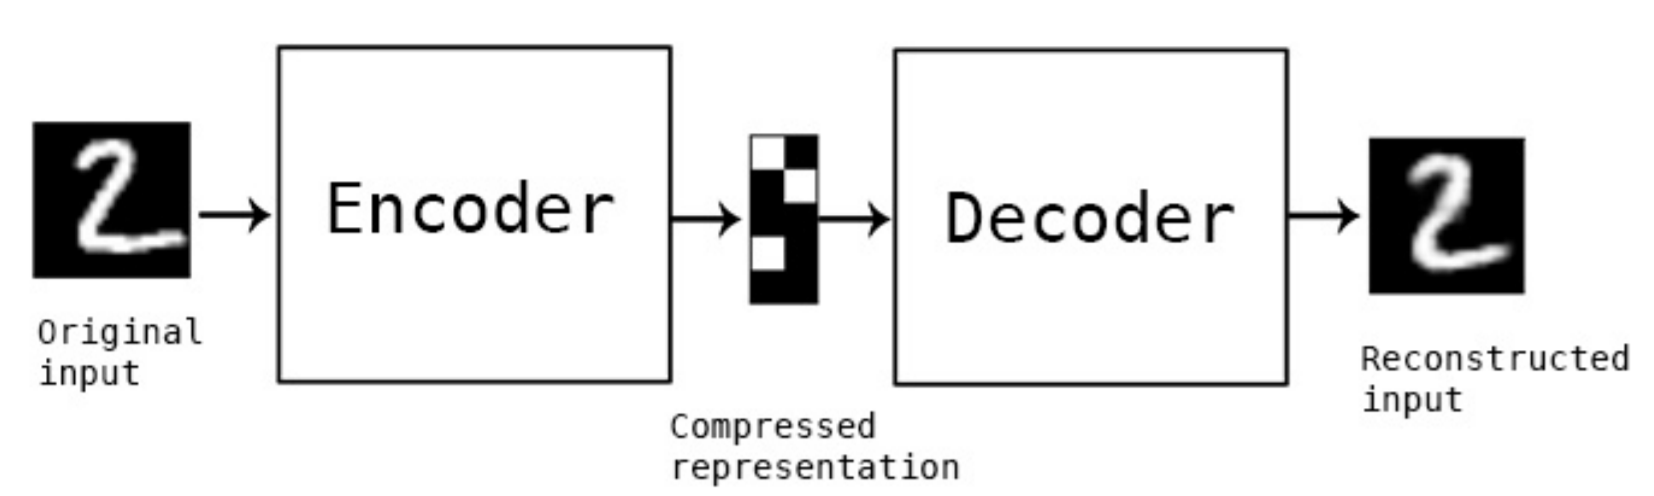
\includegraphics[width=0.9\textwidth]{img/autoencoder.PNG}
    \caption{Overview of an Autoencoder. The Autoencoder is composeb by two modules: the \textbf{encoder} module transforms the original pattern into a compressed representation. This representation is a compressed version of the original input. The \textbf{decoder} module takes the compressed representation and tries to reconstruct the original pattern. Adapted from \cite{chollet2016building}.}
\label{fig:autoencoder}
\end{figure}

The AE is a traditional feed-forward ANN that trains with back-propagation, but it employs an \textit{unsupervised learning} algorithm. While most ANNs require labeled data to train (supervised learning), the AE eliminates the need for labels by using the training patterns as both the inputs and the targets in the training process. The fact that the input and the targets (which are the desired outputs) are equal, means that the neural network's goal is to learn to copy what it receives in the input layer onto the output layer \cite{bengio2017deep}.

For an AE to be a useful compression tool, we must ensure that:
\begin{itemize}
    \item The representations $h$ are compressed, i.e., they have considerably less information capacity when compared with the original input.
    \item The decoder module must be able to transform the compressed representations back into close reconstructions of the original input.
\end{itemize}

The first aspect ensures that the encoder will learn a compression function, and it is addressed when designing the network.
The hidden layer in between the encoder and decoder must act as an information bottleneck.
There are many ways to implement the information bottleneck. Depending on the application, different properties will be enforced in the representations. For example, \textit{undercomplete} AEs have a very small hidden layer; regularized AEs (Sparse, Denoising, or Contractive) add penalty terms to the loss function \cite{vincent2010stacked}.

The second aspect ensures that the compression is not excessively lossy. If the reconstruction accuracy remains low after training, it means that the information bottleneck is too restrictive. Contrarily, if the AE has a good reconstruction accuracy after training, it means that the compression rate is adequate, and the AE is learning compressed representations that capture the relevant features of the patterns.

It is important to underline how the ANN's accuracy is interpreted in AEs, as it is quite different from typical ANNs. In a traditional ANN task, such as the classification of MNIST digits \cite{lecun1998mnist}, a solution is as good as its accuracy. The goal is to create a network that can classify novel examples with 100\% accuracy. Researchers try out many different architectures and train them endlessly with backpropagation to obtain the best possible score. 
With AEs, perfect accuracy is not the goal. The network accuracy of an AE tells us how well the decoder module can reconstruct the original pattern. Since the AE is a lossy compression algorithm, the decoder cannot generate perfect reconstruction, even with extensive training. The best possible accuracy of an AE will be bounded by the compression factor imposed by the architecture. Therefore, the accuracy of an AE should be seen as an indicator of the "lossy-ness" of the compression and not the quality of the solution.

%example 
Let us look at a simple example that illustrates the role of accuracy in AEs: Suppose we want to compress images of $10 \times 10$ pixels and we have three possible architectures:
\begin{enumerate}
    \item Use an AE that has a hidden layer with 10 units. After training it manages to create reconstructions with 60\% accuracy.
    \item Use an AE that has a hidden layer with 100 units (as many units as pixels). After training it manages to create reconstructions with 100\% accuracy.
    \item Use an AE that has a hidden layer with 20 units. After training it manages to create reconstructions with 95\% accuracy.
\end{enumerate}

The first AE is the one with the highest compression rate, but this comes at the cost of a big loss in the reconstruction accuracy. The compression is too lossy.

The second AE is useless: by having as many units as pixels, the network can learn how to simply copy its input with the identity function. No compression is performed.

The third AE is the best option. It manages to reduce the size of the images by a factor of five and then can reconstruct the original pictures with 95\% accuracy.

With this example, we can see how there is a trade-off between compression rate and reconstruction accuracy. We can also see how the goal of an AE is not to have 100\% accuracy. When a good balance between "lossy-ness" and compression rate is achieved, the AE has learned how to extract the relevant features of the patterns and compress them into informative representations.
\newline

The AE was originally proposed as a data compression algorithm, but as François Chollet, author of the Keras library, puts it, AEs are not the best tool for data compression \cite{chollet2016building}. In picture compression, for instance, JPEG will yield much better results and will work for any domain, while the AE will only be able to compress images similar to those it trained on.
But the AE has had great success in a variety of applications other than data compression.
An important breakthrough for AEs was the technique developed by Hinton, where AEs were stacked on top of each other to learn hierarchical representations of images \cite{krizhevsky2011using}.
The two most successful applications of classical AEs are data denoising \cite{cho2013simple}  and dimensionality reduction for data visualization \cite{hinton2006reducing}.
More complex AE architectures have emerged recently. Variational AutoEncoders (VAEs) \cite{kingma2013auto} are used to learn the probability distribution of the input data, and can be used as \textit{generative models}. The domain-dependent nature of AEs can be leveraged for anomaly detection tasks \cite{sakurada2014anomaly,an2015variational}. If the AE is of the overcomplete type (with large, sparsely activated hidden representation) it can be used to generate SDRs. We will focus on the latter application in the next section.

\subsubsection{Autoencoders for the generation of SDRs}
\label{sec:prescriptions_AEs_sparse}

"An autoencoder that has been regularized to be sparse must
respond to unique statistical features of the dataset it has been trained on, rather than simply acting as an identity function." \cite{bengio2017deep}.

As we have seen previously, SDRs owe their informative nature to the strict properties of sparsity and distribution. As it turns out, these properties of SDRs can also be used as the information bottleneck of AEs. If we do so, the AE can be used to transform real-world data into SDRs.

So how exactly do we impose the properties of SDRs onto the hidden representation of an AE? We must ensure that:
\begin{enumerate}
    \item \textbf{Size}: Real-world data typically has fewer dimensions in its raw format when compared with its SDR counterpart ($\|x\| \ll \|h\|$). For this reason, the AEs that generate SDRs are usually of the \textit{overcomplete} type, where the hidden layer is larger than the input/output layer.
    
    \item \textbf{Sparsity}: To prevent the hidden layer from learning the identity function, we force the AE to learn representations that sparsely activate its hidden units (an active unit has an output close to 1). To do so, we add a penalty term to the loss function that penalizes representations that have a sparsity away from the desired value.
    
    \item \textbf{Distribution}: The AE should also learn distributed representations, i.e., it should use all of its hidden units evenly across the entire dataset. Ideally, the activation of units in the hidden layer follows a uniform probability distribution.
\end{enumerate}

Notice how the second and third properties can be combined into a single constrain: If we force all the hidden units of an AE to have approximately the same (low) activity level $\rho$ (let us say each hidden units should only activate in $\rho=2\%$ of all the patterns across a training set), we are ensuring both the sparsity and distribution property the same time.

To implement this constraint, let us define $\hat{\rho}_{j}$ as the average activation of hidden unit $j$ (averaged over the training set) \cite{ng2011sparse}:

\begin{equation}
    \hat{\rho}_{j}=\frac{1}{m} \sum_{i=1}^{m}\left[a_{j}^{(2)}\left(x^{(i)}\right)\right],
\end{equation}
where $m$ is the number of training examples, and $a_{j}^{(2)}\left(x\right)$ is the activation of hidden unit $j$ given input $x$.

If we want to generate SDRs with a sparsity level of $\rho$, then we should ensure that $\hat\rho_{j}=s \mid j=1, \dots,h$

To do so, we add a penalty term $\Omega(\rho)$ to the loss function $L$ of the AE:
\begin{subequations}
    \begin{equation}
        L_{new} = L(x,r) + \Omega(\rho)
    \end{equation}
    
    \begin{equation}
    \label{eqn:KLdiv}
        \Omega(\rho) = \mathrm{KL}\left(\rho \| \hat{\rho}_{j}\right) =  \sum_{j=1}^{h} \rho \log \frac{\rho}{\hat{\rho}_{j}}+(1-\rho) \log \frac{1-\rho}{1-\hat{\rho}_{j}},
    \end{equation}
\end{subequations}

where $h$ is the number of hidden units, and $j$ is used to iterate over all hidden units. Here, $\mathrm{KL}\left(\rho \| \hat{\rho}_{j}\right)$ is the  Kullback-Leibler (KL) divergence \cite{kullback1951information}. The KL divergence measures the distance between two density distributions. Therefore, by using $\mathrm{KL}\left(\rho \| \hat{\rho}_{j}\right)$ as a penalty term, we are rewarding the AE for generating representations that activate their units following a normal distribution $\rho$ (see figure \ref{fig:KL}).

\begin{figure}[h]
    \centering
    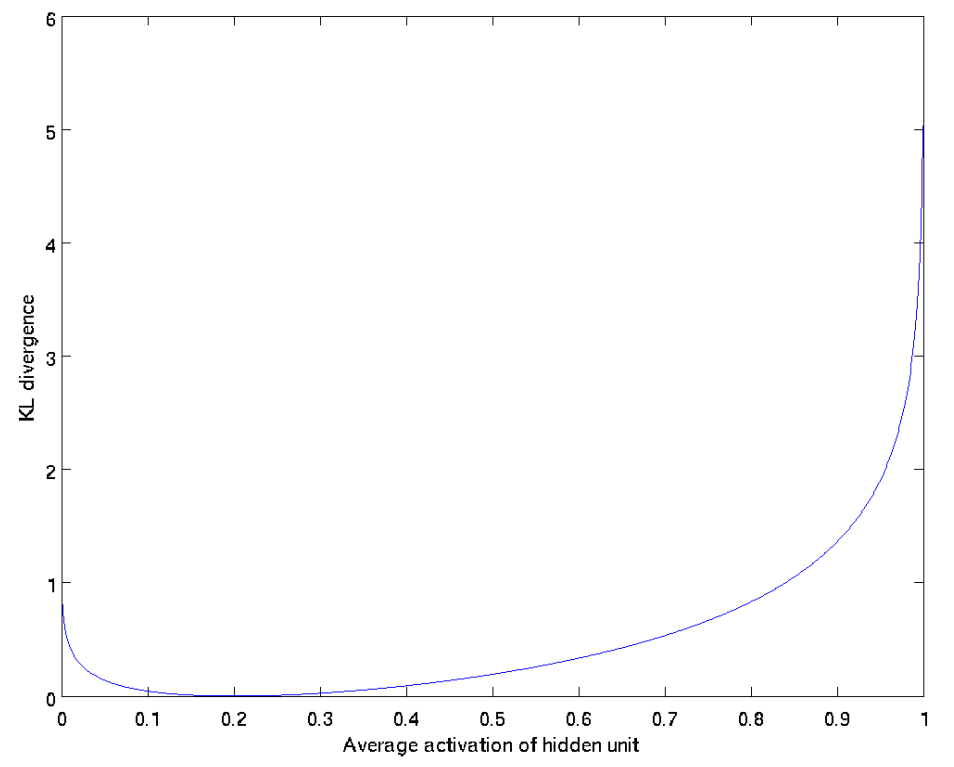
\includegraphics[width=0.65\textwidth]{img/KL.PNG}
    \caption{Example of the KL divergence. Here we want to enforce a sparsity level of $\rho = 0.2$. The KL divergence will measure the distance between the distribution $\hat\rho_j$ and the desired uniform distribution $\rho = 0.2$. Notice the global minimum when $\hat\rho_j = \rho = 0.2 $. The KL divergence will monotonically increase as we move away from $\rho$, and it explodes to $\infty$ when $\hat\rho_j$ goes to either $0$ or $1$. Adapted from \cite{ng2011sparse}.}
\label{fig:KL}
\end{figure}

After training, we can take the encoder module of a trained AE that implements these restrictions and use it to transform the trainning data into SDRs. Also, the encoder should be able to generalize to novel patterns of the same domain.

\subsection{The biology of Encoding Functions}
\label{sec:prescriptions_bio}
One might ask: ``If Associative memories are biollogically plausible, why is their performance on raw data poor? The brain handles raw data just fine." This is a valid comment, and in this section I will give a hint on the motivation behind encoding prescriptions.

Representing human knowledge on a computer has proven to be a difficult task. The problem stems from the fact that our knowledge of the world is not well-organized. Every rule has exceptions and every fact links to numerous others. This level of complexity is not well-suited for traditional computer data structures. In contrast, our brains seem to deal with this complicated knowledge with ease. Our brains do not use dense representations like those used in computers. Instead, they represent knowledge with the sparse activation of its billions of neurons. The brain uses SDRs to encode knowledge \cite{Hawkins-et-al-2016-Book}. One might ask: If real-world data, like images, is dense, how can the brain use SDRs? Indeed, sensory data is not naturally found in the form of SDRs. But we know that our brain has lower functional regions that process the inputs from the senses and generate sparse and distributed activation of neurons in the neocortex. For instance, the visual area of the brain is divided into several hierarchical regions: V1, V2, V4, and IT. The V1 area of the brain is responsible for detecting low-level visual features such as edges, and basic color. The detection of such features results in the activation of a collection of neurons that forms a signal. This signal is passed onto the V2 area which will apply a similar process. After passing through all the regions, the final result will be an SDR that represents what we are sensing \cite{hawkins2004intelligence}. Another example is auditory perception. The sounds that we hear are captured in the cochlea. The cochlea is an organ that has several receptors for different frequencies. A particular sound will result in the sparse activation of the receptors which will result in an SDR.

All-in-all there is a biological analogy between SDR encoders used for Associative memories and biological organs that transform sensory data into sparse neuron activity in biological memories.

\section{Pattern Generation}
\label{sec:gen}
In this section we present two tools that have the ability to generate patterns.

Despite some minor nomenclature disagreements, machine learning models can be divided into \textbf{Discriminative} and \textbf{Generative} \cite{ng2002discriminative,kingma2019introduction}. 

Consider a classification task with a set of examples $X$, and their corresponding labels $Y$.
A \textit{discriminative} classifier will either learn a direct mapping between $X$ and $Y$, or learn the \textit{posterior} probability of $Y$ given $X$ ($P(Y \mid X)$).
On the other hand, a \textit{generative} model has an intermediate step that learns the \textit{likelihood} of $Y$ given a fixed $X$ ($L(Y \mid X) = P(X \mid Y)$), and then learns a model of the underlying \textit{joint} probability of the data ($P(X ,Y)$).

The \textit{generative} model's task is a  much more general and difficult one. By learning the \textit{joint} distribution, it is also possible to compute the \textit{posterior} with Bayes Rule ($P(Y \mid X)=\frac{P(X \mid Y) \cdot P(Y)}{P(X)}$). Contrarily, a \textit{discriminative} model that has leaned the posterior, isn't able to infer the joint.
In the context of pure classification tasks, using generative models is traditionally seen as overkill \cite{vapnik2013nature}, but the added complexity of the \textit{generative} tasks allows the model to go beyond classification: a trained generative model can generate new artificial examples drawn from the distribution of the data, hence the name \textit{generative}.

\subsection{Variational Autoencoders}
\label{sec:gen_VAE}
As we saw in section \ref{sec_AEs}, the traditional AE compresses its inputs $x$ into  feature vectors $h$. These feature vectors are simply an array of real values that represent the presence of latent features in the inputs.

Variational Autoencoders (VAEs) extend the basic AE architecture by representing the probability distribution functions of the latent features, as opposed to simply representing their value. For instance, if we assume that the features follow a normal distribution, the hidden layer of a VAE would represent the mean and standard deviation for each dimension of the hidden space. The goal of a VAE is to learn the posterior distribution \(P(Z \mid X)\) over a set of unobserved variables $Z$, given some data $X$. Computing the exact value for the posterior is often intractable since it requires the computation of \(P(X)=\int_{}^{} P(X \mid Z)P(Z) \,dz\) over all the dimensions of $z$. VAEs circumvent this problem with \textit{variational inference}, i.e. the model learns an approximated tractable distribution of the posterior: \( Q(\mathbf{Z}) \approx P(\mathbf{Z} \mid \mathbf{X})\). To ensure that $Q$ is a good approximation of the real distribution, we can minimize the KL divergence (eq. \ref{eqn:KLdiv}) between them.

The VAE is implemented as two independently parameterized networks that work together: the encoder/recognition model and the decoder/generative model \cite{bengio2017deep}. These two models train together with back-propagation, where the loss function simultaneously maximizes the reconstruction likelihood and minimizes the KL divergence between the approximation and the unknown distribution:

\begin{equation}
    loss = E_{Q(Z \mid X)} \log P(X \mid Z)-K L(Q(Z \mid X) \| p(Z)),
\end{equation}
where  \(E_{Q(Z \mid X)}\) is the expected value over the distribution \(Q\).
\newline

Once the VAE is trained, its weights can be fixed, and we can generate new examples by sampling from the learned distribution \(Q\) (see figure \ref{fig:VAE}).

\begin{figure}[h]
    \centering
    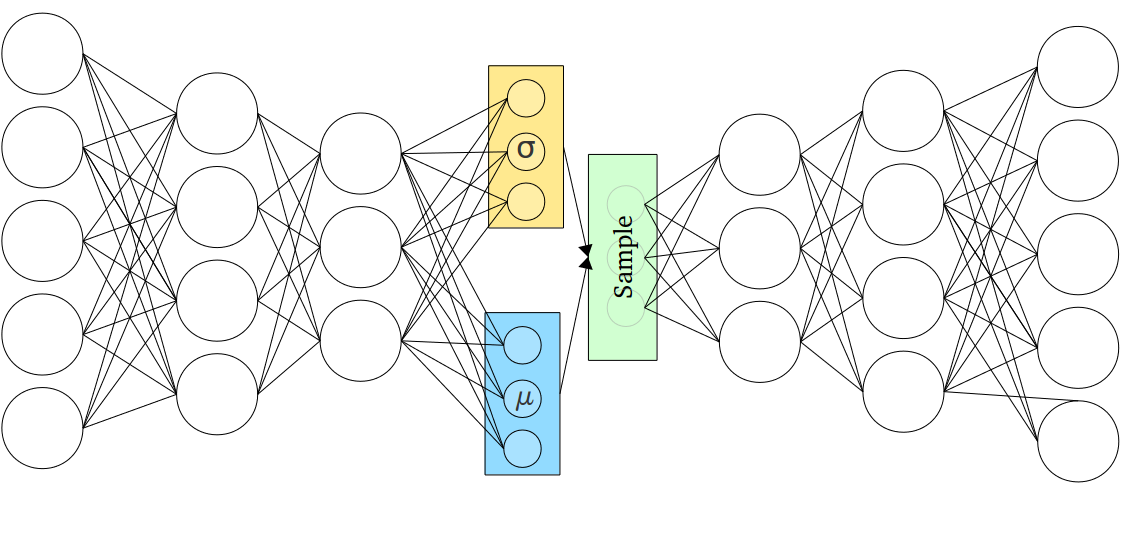
\includegraphics[width=0.8\textwidth]{introduction/img/VAE.png}
    \caption{Architecture of a VAE. The network on the left is the encoder/recognition module which models \(Q(Z \mid X)\); In the middle, the hidden compression of this AE corresponds to the normal distribution of three latent features, i.e. three means (in blue), and three standard deviations (in yellow); The approximated distribution is randomly sampled (in green); The network on the right is the decoder, which models \(P(X \mid Z)\). Adapted from \cite{shafkat2018VAE}.}
\label{fig:VAE}
\end{figure}

\subsection{Generative Adversarial Networks}
\label{sec:gen_GANs}
Generative Adversarial Networks (GANs) are a family of generative models that combine ideas from Game Theory and Machine Learning. A GAN consists of two independent neural networks that are trained simultaneously with back-propagation: a generative model $G$ that learns the distribution of the original data, and a discriminative model $D$ that learns to distinguish between fake patterns generated by $G$ and real patterns from the original dataset \cite{goodfellow2014generative}.

The training process of a GAN is an adversarial minimax game between the two models. The goal of $G$ is to fool $D$ into thinking that its patterns are real and the goal of $D$ is to distinguish between real and fake patterns. As the two models compete, they gradually improve at their tasks. The game will eventually reach a \textit{Nash equilibrium}, where $G$ has implicitly captured the correct probability distribution of the data, and $D$ can't do better than random guessing since both the fake and real patterns appear to come from the same distribution.

After training, the two models can be decoupled and used independently. The Discriminator's most common applications are classification in semi-supervised learning scenarios \cite{salimans2016improved}, and domain adaptation \cite{bousmalis2017unsupervised}.
The Generator module is used to generate new patters. A \textit{seed} provided in the input layer will determine the resulting pattern. The basic use-case of the Generator is to provide \textit{random noise} as the \textit{seed} to obtain a pattern similar to those in the training set. More advanced use cases involve operations between \textit{seeds}. Since the generation process is deterministic (a seed will always output the same pattern), a GAN can utilize vector arithmetic and interpolation to obtain complex patterns. For instance it is possible to interpolate between two classes as seen in figure \ref{fig:GANS_interp}.

\begin{figure}[h]
    \centering
    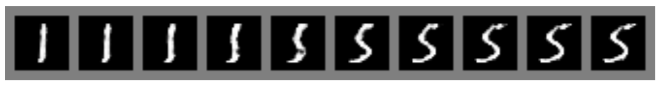
\includegraphics[width=0.5\textwidth]{introduction/img/GANS_interp2.PNG}
    \caption{Pattern interpolation with a Generative Adversarial Network (GAN). Here a GAN was trained on the MNIST dataset of hand written digits \cite{lecun1998mnist}. If we take the seed that generates the image of a "one", and the seed that generates the image of a "five", we can interpolate between the two seeds to obtain a transformation in the image space. Adapted from \cite{goodfellow2014generative}.}
\label{fig:GANS_interp}
\end{figure}

\section{Proposed Solution}
\label{sec:proposedSolution}
\subsection{Hypothesis}
The What-Where sparse codes developed in \cite{sa2020storing} implement an effective compression function for associative memories, but a decompression module that would allow for interpretability is missing. My research goal is to build the aforementioned decompression module. I hypothesize that autoencoders could be used to complete this task since they simultaneously implement an encoding and decoding function.
\subsection{Data Description}
The MNIST dataset \cite{lecun1998mnist} of hand-written digits will be used. This dataset consists of 60,000 labeled examples with an equal number of examples for each of the ten classes (digits zero to nine). Not only is this dataset a popular benchmark for the AI community, but it was also the dataset used in the previous research that leads up to my dissertation.

\subsection{Experiments}
\label{sec:proposedSolution_exp}
%The starting point of the experiments is the already-implemented compressor in figure %\ref{fig:archi_start}.
%\begin{figure}[h]
%    \centering
%    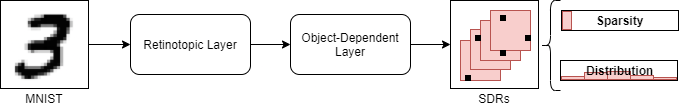
\includegraphics[width=0.99\textwidth]{introduction/img/archi_start.png}
%    \caption{Architecture of starting point.}
%\label{fig:archi_start}
%\end{figure}

To transform sparse codes into visual reconstructions in mind, I plan to the following experiments of increasing complexity:
\begin{enumerate}

    \item \textbf{Establish the architecture of the models}: The architecture of the autoencoder variants must be tweaked to prevent overfitting or underfitting on the dataset. Simple solutions that can be coded from scratch will be proffered. However, if a complex model is required, libraries such as \textit{pytorch} will be used. In any case, deep-learning-like fine-tuning will be averted.
    Some of the hyper.parameters that I plan to go over are:
    \begin{itemize}
        \item Number of Hidden Layers.
        \item Number of Hidden Units.
        \item Convolution and/or Deconvolution Layers.
    \end{itemize}
    
    \item \textbf{Decompression as pseudo-generation}: Use a trained AE to decompress the SDRs into visual patterns.
    
    \begin{itemize}
        \item Guide the training of an AE so that its hidden layer shares the properties of SDRs (sparsity and distribution). This is achieved by changing the learning rule as described in eq. \ref{eqn:KLdiv}.
        \item Use the decoder module of the AE to transform the sparse codes into decompressions.
    \end{itemize}
    \item \textbf{Generation}: Use generative models (variational autoencoders) to transform the sparse codes into new patterns.
    \begin{itemize}
        \item Train a VAE where the hidden layer has the same properties as the SDRs.
        \item Sample from the learned distributions of the  VAE's hidden layer to generate images.
    \end{itemize}


\end{enumerate}

\subsection{Evaluation Method}
% WE ARE BUILDING RECONSTRUCTIONS
The first step in my project is to build autoencoders that approximate the encoding function of the What-Where sparse codes.
Given an autoencoder that transforms a training set $\mathbf{X}$ into a hidden set $\mathbf{H}$, and the What-where codes $\mathbf{C}$, the quality of the approximation is given by:
\begin{itemize}
    \item The difference between the sparsity of $\mathbf{H}$ and $\mathbf{C}$.
    \item The KL-divergence between the approximation and the What-Where codes: $\mathrm{KL}\left(\mathbf{H} \| \mathbf{C}\right)$.
\end{itemize}

Then we focus on transforming the What-Where sparse codes back into images.
Evaluating the solution will boil down to a quantitative and qualitative evaluation of the reconstructions.

Given a training set $\mathbf{X}$, and the What-Where sparse codes $\mathbf{C}$, the goal is to transform $\mathbf{C}$ into reconstructions $\mathbf{X}^{\prime}$, that are similar to $\mathbf{X}$.
We can evaluate the solution by:
\begin{itemize}
    \item Measuring the mean squared loss: $\mathcal{L}\left(\mathbf{X}, \mathbf{X}^{\prime}\right)=\left\|\mathbf{X}-\mathbf{X}^{\prime}\right\|^{2}$.
    \item Measuring the classification accuracy of GAN trained on $\mathbf{X}$.
    \item Measuring the classification accuracy of a 1 nearest-neighbor classifier that trains on $\mathbf{X}$ and classifies $\mathbf{X}^{\prime}$.
\end{itemize}
%THIS IS HOW WE MEASURE RECONSTRUCTION LOSS
Since the What-Where sparse codes are lossy compressions, imperfect reconstruction is expected. For this reason, a qualitative evaluation of the reconstructions will be done. Reconstructions that look like vague/incomplete versions (see figure \ref{fig:imperfect_recon} for a visual explanation) of the original patterns would be an exciting result.

\begin{figure}[h]
    \centering
    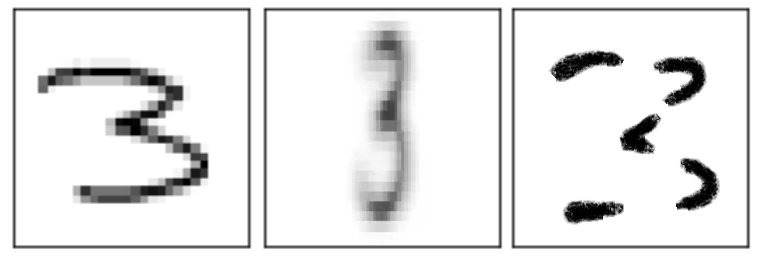
\includegraphics[width=0.6\textwidth]{introduction/img/result_prediction.png}
    \caption{Expected imperfect reconstructions. \textbf{(left)} A pattern from the original dataset. \textbf{(center)} A reconstruction that looks like the average example of the class. \textbf{(right)} A reconstruction that has the prime features of the training example but is missing some details.}
    \label{fig:imperfect_recon}
\end{figure}

\section{Tentative Schedule}
\label{sec:schedule}
Here we present how the work for the Master Thesis in the next semester will be structured.
Writing (the Dissertation and possibly a scientific paper) will be highly valued since putting ideas into written form helps in doing proper scientific research. Figure \ref{fig:schedule} depicts the work that has been done so far in the Project course and outlines the work for next semester.  
\begin{figure}[h]
    \centering
    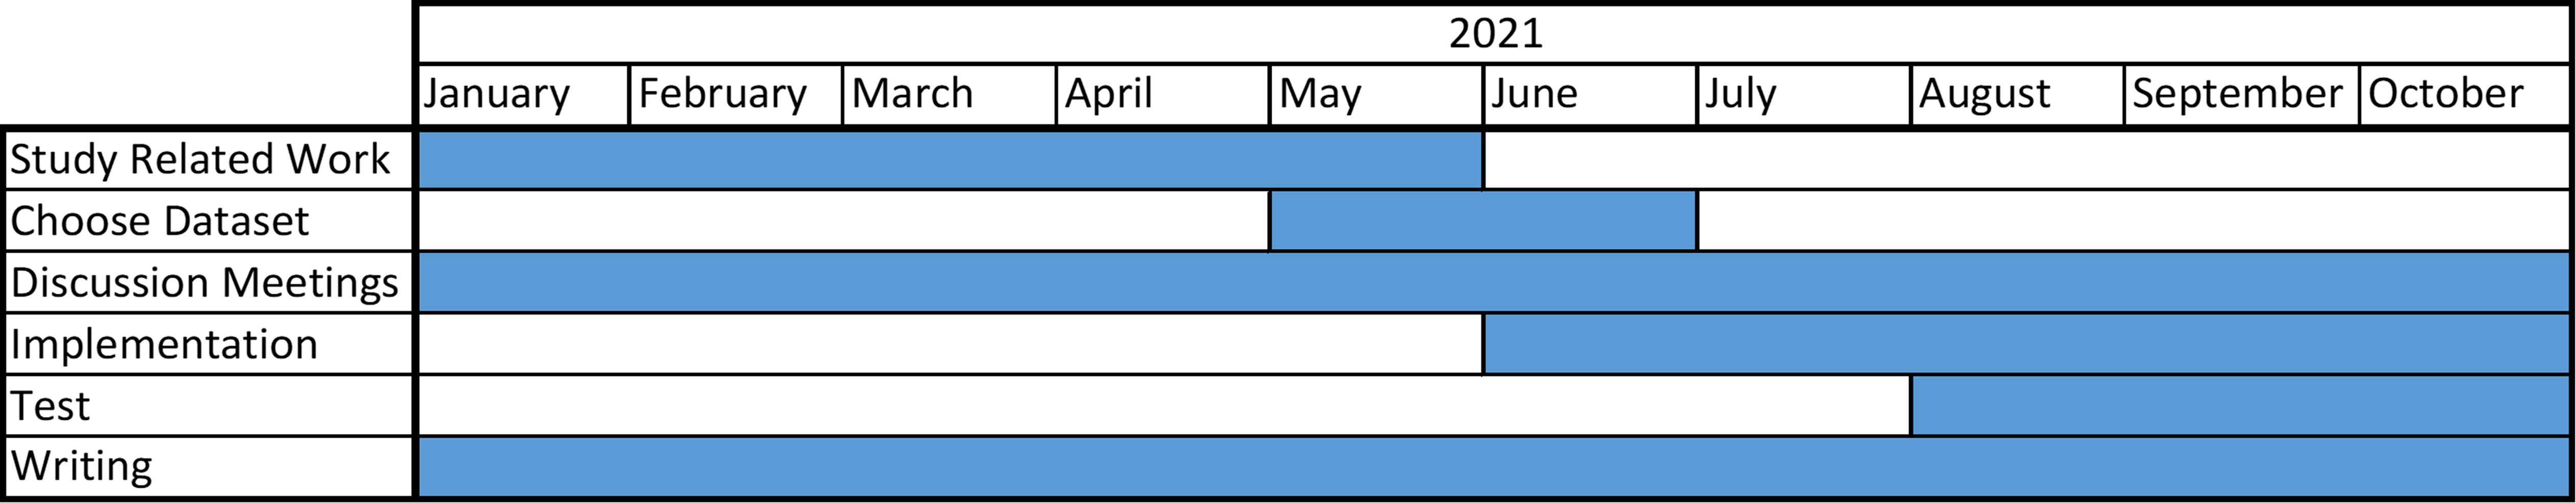
\includegraphics[width=0.99\textwidth]{introduction/img/schedule.png}
    \caption{Tentative Schedule.}
    \label{fig:schedule}
\end{figure}

\section{Conclusion}
\label{sec:conclusion}
The goal of Artificial Intelligence is to build systems with human or even super-human-like intelligence. Since the brain is the most intelligent system that we know of, I believe that it is useful to study \textit{Biollogically-Inspired Models}. One example of such models is the \textit{Associative Memory} (AM) (section \ref{sec:assomem}): a family of mathematical models that stores and recalls information similarly to biological memories. A major roadblock of AMs is the so-called \textit{Sparse Coding Problem} (section \ref{sec:inputoutput_problem}) which also affects other research domains. To solve this problem, sparse encoding prescriptions that transform raw data into sparse codes are required.
In my thesis, I will study one such prescription (section \ref{sec:prescriptions_WW}), which has successfully been applied to Willshaw Networks (section \ref{sec:wn}). This prescription performs feature extraction of visual patterns and generates lossy sparse compressions. The goal of my thesis is to ``see" these compressions, that is, develop a mechanism that can map the compressions back into the visual space of the original patterns. Reconstructing the compression will help us to better understand the success of the encoding prescription, and give us hints on how to successfully apply AMs in practice.
To fulfill my research goal I plan to use Autoencoders (section \ref{sec:prescriptions_AEs}) and its several variants (sections \ref{sec:prescriptions_AEs_sparse}, and \ref{sec:gen_VAE}) on the MNIST dataset of hand-written digits (proposed experiments in section \ref{sec:proposedSolution}).

To conclude, a tentative schedule that maps the work to be done next semester is presented (section \ref{sec:schedule}).


\bibliographystyle{splncs04}
\bibliography{refs}

\end{document}